\chapter{Experiments}
\label{chapter:experiments}


\section{Full Lap Planning Test}

In this experiment we will test the Hybrid A* and \gls{SEHS} algorithms as we described them in Section~\ref{sec:trajectory_planning_algorithms} on several different circuit maps. For each circuit, their task will be to find a near time-optimal trajectory from a starting position through a series of waypoints until the last waypoint of the circuit is reached. We will then compare the quality of the solutions, how much of the state space the algorithm had to explore before it found the solution, and how long it took to calculate the result.

\subsection{Test Setup}

The parameters of the vehicle chassis and the vehicle model we used are equal to the properties of our experimental vehicle as stated in Table~\ref{table:dimensions} and derived in Section~\ref{sec:actuators_model}.

Both Hybrid A* and \gls*{SEHS} require specification of state space and time discretization parameters. We found that both algorithms performed well with time step $\Delta t=\SI{0.04}{\second}$ (\SI{25}{\hertz}), the heading angle values divided into \num{24} sectors of a circle, and the range of possible values of motor \gls*{RPM} divided into \num{50} sub-ranges. Additionally, the Hybrid A* algorithm splits the $x$ and $y$ coordinates were split into squares with side lengths of $4r$, where $r$ is the radius of the vehicle. The SEHS algorithm discretizes the $xy$ plane by finding a path of circles in the Space Exploration step. We require the radii of the circles to be between $r$ a $5r$.

The actions available to the planner were a cross product of 5 throttle levels (\num{-1}, \num{-0.5}, \num{0}, \num{0.5}, \num{1}) and 11 target steering angles (\num{-1}, \num{-0.8}, \num{-0.6}, \num{-0.4}, \num{-0.2}, \num{0}, \num{0.2}, \num{0.4}, \num{0.6}, \num{0.8}, \num{1}). This limits the possible maneuvers of the vehicle, but it allows the planner to run reasonably fast.

Circuits are represented by an occupancy grid bitmap with a resolution of \SI{0.05}{\meter} per grid cell. For each circuit, we first perform track segmentation, as described in Section~\ref{sec:track_segmentation}, to detect corners which we use as waypoints. We also perform the Space Exploration step of the SEHS algorithm. We then let both algorithms find the near time-optimal trajectory from the initial configuration defined for each circuit to the last waypoint. We measure the number of search nodes the algorithm opens during search, the number of search nodes which are expanded, and also the time it takes to find the solution on a testing computer. Because both of the algorithms are deterministic, they always find the same solution for the same problem and they always open and expand the same number of search nodes. The execution times differ slightly and so we repeat the measurement 100 times and calculate the mean execution time.

We used a desktop computer with an AMD Ryzen 7 3700X CPU running at the base clock of \SI{3.6}{\giga\hertz} and \SI{32}{\giga\byte} of DDR4 RAM at the base clock of \SI{3200}{\mega\hertz}. The source code was written in C++ and compiled using GCC 9.2 with the \texttt{-O3} and \texttt{-ffast-math} optimization flags. We ran each planning algorithm 50 times for every circuit to calculate the average computation time using our testing computer.

\subsection{Results}

The results of our experiments are shown in Figure~\ref{fig:porto},~\ref{fig:tornado},~\ref{fig:simple},~\ref{fig:u}, and~\ref{fig:zurich}.

Each figure shows the trajectory as a red curve from the initial configuration (marked with a green arrow) to a final configuration which passes the last waypoint (marked with a red waypoint). The black stars along the trajectory are a visual aid which marks the position of the vehicle every 1 second. The waypoints found by the track segmentation algorithm are marked as blue circles.

The trajectory is plotted over a map of the circuit with white parts showing the road and gray parts the boundaries of the track. As we mentioned earlier, the occupancy grids for the circuits all have resolution of \SI{0.05}{\meter}. Every \num{20} grid cells correspond to \SI{1}{\meter} in real world. Therefore for example the circuit in Figure~\ref{fig:zurich} represents an area of \SI{25}{\meter} $\times$ \SI{25}{\meter}.

Each trajectory is accompanied by three charts, showing the control inputs for the vehicle, the normalized state of the actuators, and the speed profile of the trajectory.

\todo[inline]{Add commentary for the results.}


\begin{figure}[!tbp]%
	\centering

	\begin{subfigure}[t]{\textwidth}
		\begin{subfigure}[t]{0.45\textwidth}
			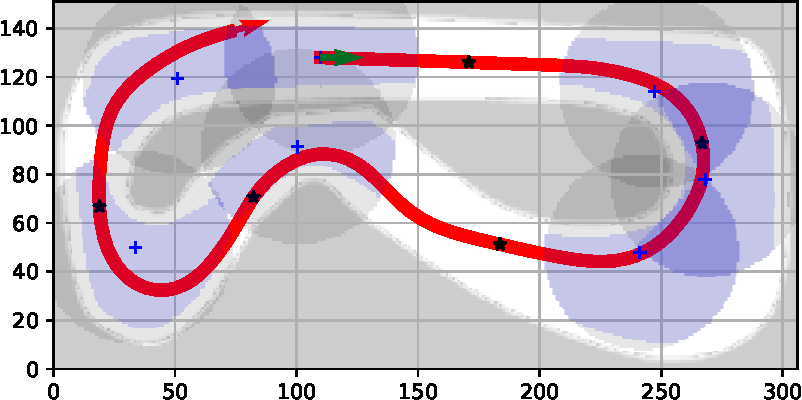
\includegraphics[width=\textwidth]{../img/experiments/porto-hybrid_astar-trajectory}
		\end{subfigure}
		\hfill
		\begin{subfigure}[t]{0.45\textwidth}
			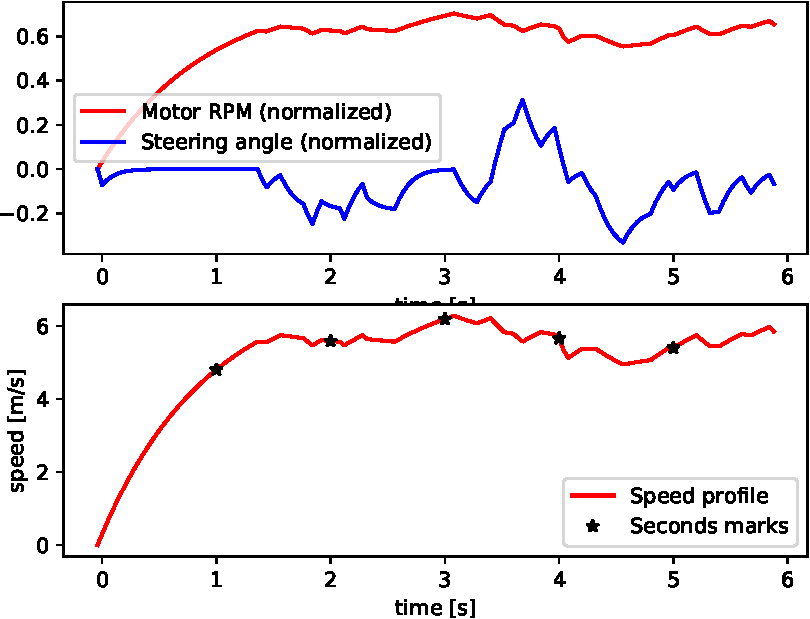
\includegraphics[width=\textwidth]{../img/experiments/porto-hybrid_astar-actuators}
		\end{subfigure}
		\caption{Solution found by Hybrid A* in \SI{192.30}{\milli\second}}
		\label{fig:solution_porto-hybrid_astar}	
	\end{subfigure}
	
	\vspace{0.75cm}
	
	\begin{subfigure}[t]{\textwidth}
		\begin{subfigure}[t]{0.45\textwidth}
			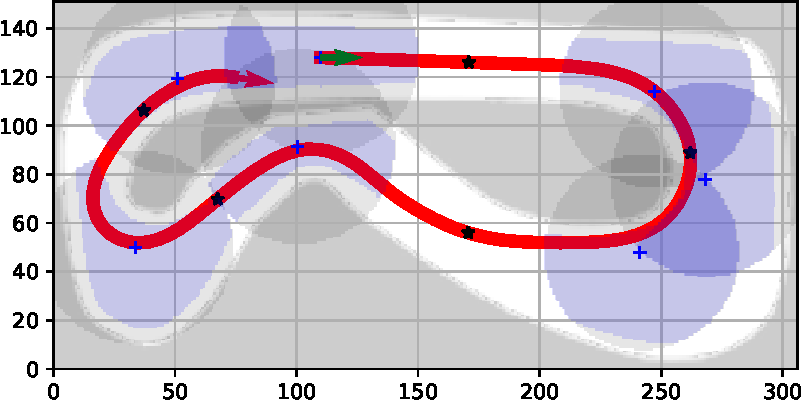
\includegraphics[width=\textwidth]{../img/experiments/porto-sehs-trajectory}
		\end{subfigure}
		\hfill
		\begin{subfigure}[t]{0.45\textwidth}
			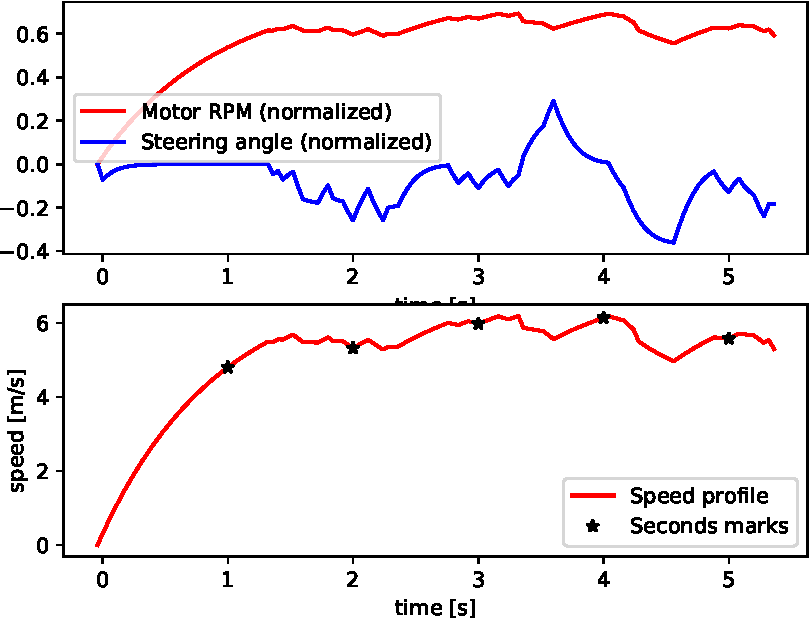
\includegraphics[width=\textwidth]{../img/experiments/porto-sehs-actuators}
		\end{subfigure}
		\caption{Solution found by SEHS in \SI{253.60}{\milli\second}}
		\label{fig:solution_porto-sehs}
	\end{subfigure}

	\vspace{0.75cm}

	\begin{subfigure}[t]{\textwidth}
		\centering
		\begin{tabular}{r r r r r r r r}%
			\toprule
			Actions & Grid cell size & RPM levels & Heading angle sectors & Opened & Expanded & Search time & Distance & Lap time \\	
			\midrule
			\num{44} & \num{1.80} & \num{20} & \num{18} & \bftab \num{67301} & \bftab \SI{192.30}{\milli\second} & \SI{39.94}{\meter} & \SI{13.64}{\second} \\
			\num{248} & \num{1.44} & \num{20} & \num{36} & \num{838926} & \SI{2544.00}{\milli\second} & \SI{36.99}{\meter} & \bftab \SI{12.28}{\second} \\
			\bottomrule
		\end{tabular}
		\caption{Hybrid A* found both a trajectory in the least amout of time and also a trajectory with the best lap time.}
		\label{table:porto-hybrid_astar}
	\end{subfigure}
	
	\begin{subfigure}[t]{\textwidth}
		\centering
		\begin{tabular}{r r r r r r r r r}%
			\toprule
			Actions & Circles & RPM levels & Heading angle sectors & Opened & Expanded & Search time & Distance & Lap time \\			
			\midrule
			\num{44} & \num{71} & \num{20} & \num{18} & \num{80763} & \SI{253.60}{\milli\second} & \SI{39.62}{\meter} & \SI{13.16}{\second} \\
			\num{84} & \num{71} & \num{80} & \num{36} & \num{1054427} & \SI{2171.60}{\milli\second} & \SI{37.50}{\meter} & \SI{12.48}{\second} \\
			\bottomrule
		\end{tabular}
		\caption{SEHS could not find a solution faster nor could it find a better solution than Hybrid A* with any of the tested combination of parameters.}
		\label{table:porto-sehs}
	\end{subfigure}
	
	\vspace{0.75cm}
	
	\caption{Circuit ``Porto''}
	\label{fig:porto}
\end{figure}

\begin{figure}[!tbp]%
	\centering
	
	\begin{subfigure}[t]{\textwidth}
		\begin{subfigure}[t]{0.45\textwidth}
			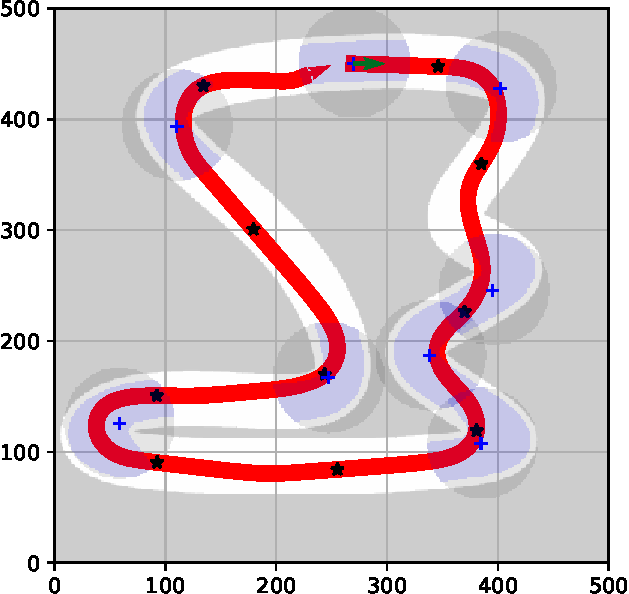
\includegraphics[width=\textwidth]{../img/experiments/tornado-hybrid_astar-trajectory}
		\end{subfigure}
		\hfill
		\begin{subfigure}[t]{0.45\textwidth}
			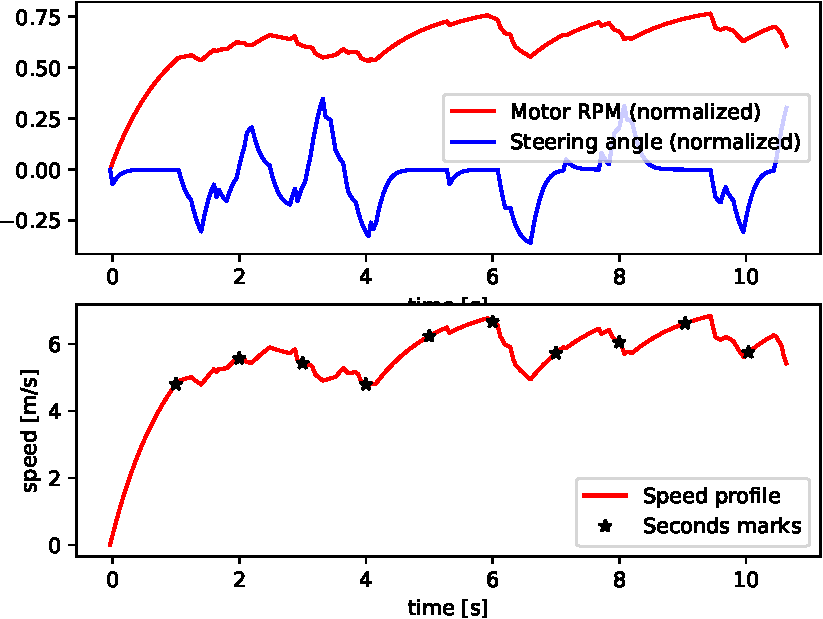
\includegraphics[width=\textwidth]{../img/experiments/tornado-hybrid_astar-actuators}
		\end{subfigure}
		\caption{Solution found by Hybrid A* in \SI{494.50}{\milli\second}}
		\label{fig:solution_tornado-hybrid_astar}	
	\end{subfigure}
	
	\vspace{0.75cm}
	
	\begin{subfigure}[t]{\textwidth}
		\begin{subfigure}[t]{0.45\textwidth}
			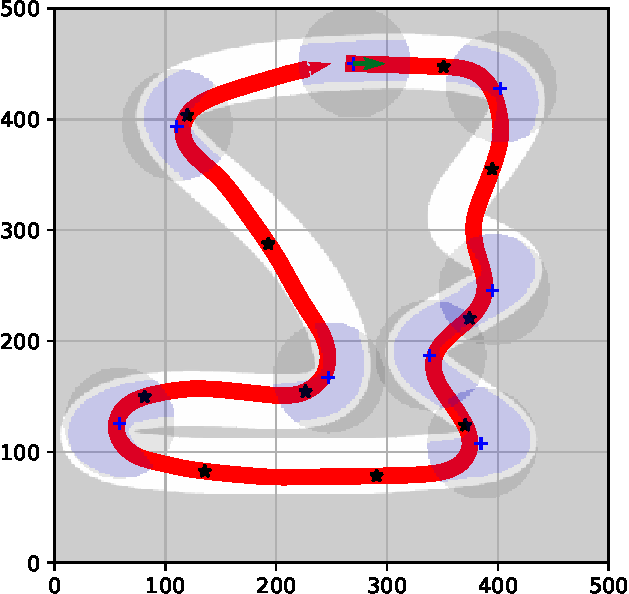
\includegraphics[width=\textwidth]{../img/experiments/tornado-sehs-trajectory}
		\end{subfigure}
		\hfill
		\begin{subfigure}[t]{0.45\textwidth}
			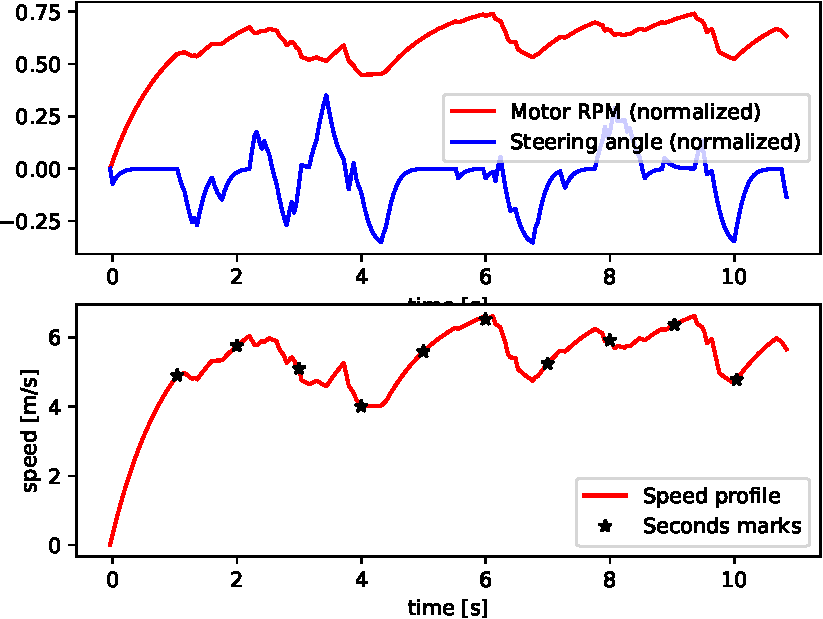
\includegraphics[width=\textwidth]{../img/experiments/tornado-sehs-actuators}
		\end{subfigure}
		\caption{Solution found by SEHS in \SI{551.30}{\milli\second}}
		\label{fig:solution_tornado-sehs}
	\end{subfigure}
	
	\vspace{0.75cm}
	
	\begin{subfigure}[t]{\textwidth}
		\centering
		\begin{tabular}{r r r r r r r r}%
            \toprule
                Actions & Grid cell size & RPM levels & Heading angle sectors & Opened & Expanded & Search time & Distance & Lap time \\
            \midrule
                \num{44} & \num{1.44} & \num{20} & \num{18} & \num{177778} & \bftab \SI{494.50}{\milli\second} & \SI{85.22}{\meter} & \SI{28.64}{\second} \\
                \num{84} & \num{1.44} & \num{80} & \num{52} & \num{3464766} & \SI{6611.70}{\milli\second} & \SI{84.96}{\meter} & \bftab \SI{26.24}{\second} \\
			\bottomrule
		\end{tabular}
		\caption{Hybrid A*: }
		\label{table:tornado-hybrid_astar}
    \end{subfigure}
    
    \begin{subfigure}[t]{\textwidth}
		\centering
		\begin{tabular}{r r r r r r r r}%
            \toprule
                Actions & Circles & RPM levels & Heading angle sectors & Opened & Expanded & Search time & Distance & Lap time \\
            \midrule
                \num{44} & \num{126} & \num{20} & \num{18} & \bftab \num{144864} & \SI{551.30}{\milli\second} & \SI{87.37}{\meter} & \SI{28.08}{\second} \\
                \num{84} & \num{126} & \num{80} & \num{52} & \num{2827948} & \SI{6397.60}{\milli\second} & \SI{84.68}{\meter} & \SI{26.84}{\second} \\
			\bottomrule
		\end{tabular}
		\caption{SEHS: }
		\label{table:tornado-sehs}
	\end{subfigure}
	
	\vspace{0.75cm}
	
	\caption{Circuit ``Tornado''}
	\label{fig:tornado}
\end{figure}

\begin{figure}[!tbp]%
	\centering

	\begin{subfigure}[t]{\textwidth}
		\begin{subfigure}[t]{0.45\textwidth}
			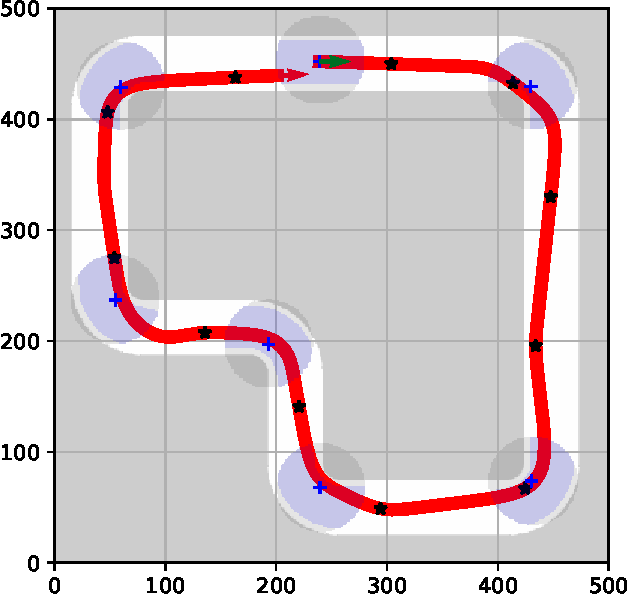
\includegraphics[width=\textwidth]{../img/experiments/simple-hybrid_astar-trajectory}
		\end{subfigure}
		\hfill
		\begin{subfigure}[t]{0.45\textwidth}
			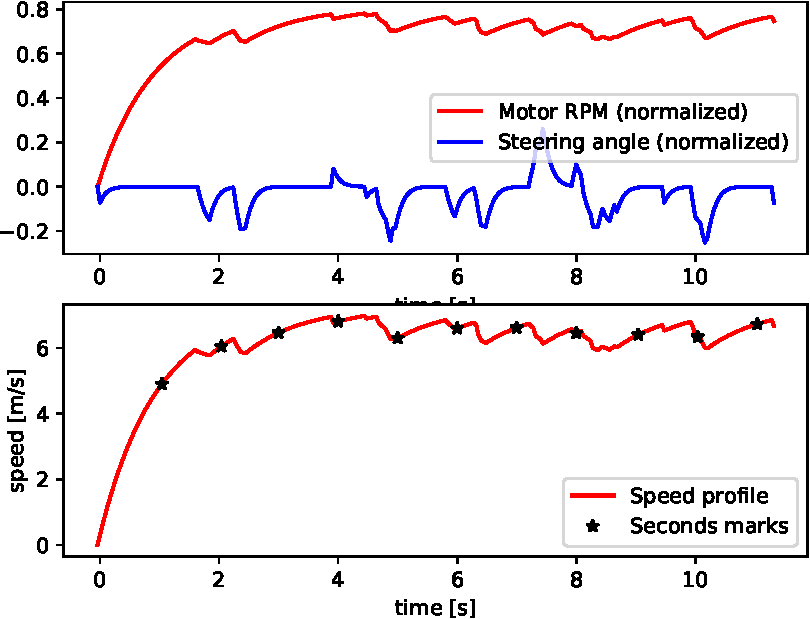
\includegraphics[width=\textwidth]{../img/experiments/simple-hybrid_astar-actuators}
		\end{subfigure}
		\caption{Solution found by Hybrid A* in \SI{236.20}{\milli\second}}
		\label{fig:simple-hybrid_astar}
	\end{subfigure}

	\vspace{0.75cm}
	
	\begin{subfigure}[t]{\textwidth}
		\begin{subfigure}[t]{0.45\textwidth}
			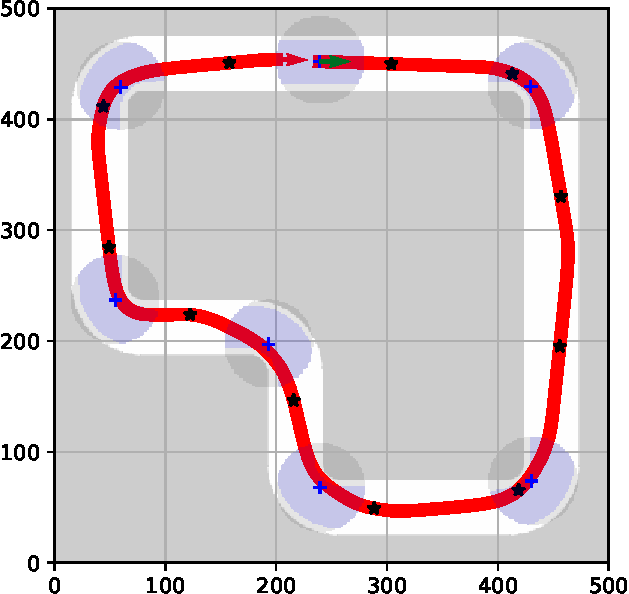
\includegraphics[width=\textwidth]{../img/experiments/simple-sehs-trajectory}
		\end{subfigure}
		\hfill
		\begin{subfigure}[t]{0.45\textwidth}
			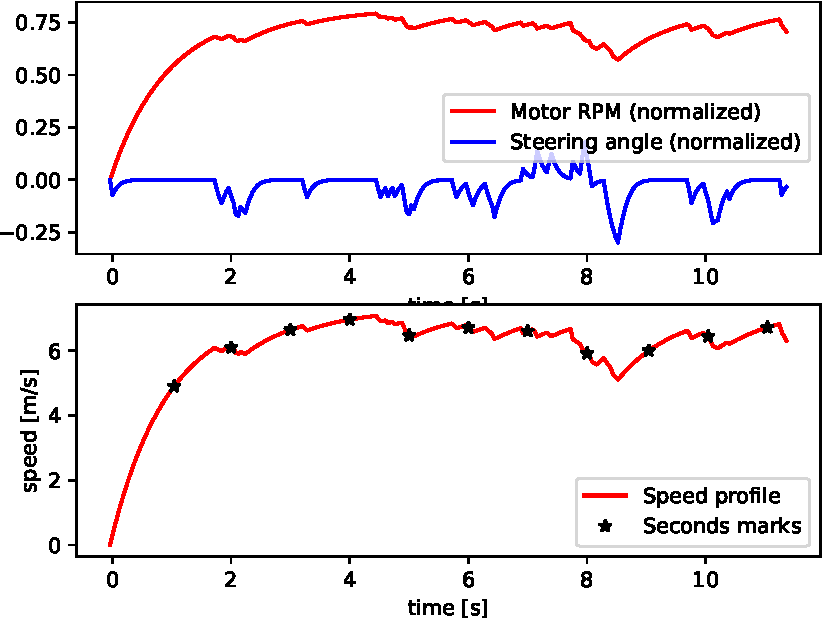
\includegraphics[width=\textwidth]{../img/experiments/simple-sehs-actuators}
		\end{subfigure}
		\caption{Soultion found by SEHS in \SI{449.20}{\milli\second}}
		\label{fig:simple-sehs}
	\end{subfigure}

	\vspace{0.75cm}

	\begin{subfigure}[t]{\textwidth}
		\centering
		\begin{tabular}{r r r r r r r r}%
			\toprule
                Actions & Grid cell size & RPM levels & Heading angle sectors & Opened & Expanded & Search time & Distance & Lap time \\
            \midrule
                \num{44} & \num{1.80} & \num{20} & \num{18} & \bftab \num{78401} & \bftab \SI{236.20}{\milli\second} & \SI{69.75}{\meter} & \SI{20.88}{\second} \\
                \num{84} & \num{1.44} & \num{40} & \num{36} & \num{807771} & \SI{1926.50}{\milli\second} & \SI{67.91}{\meter} & \SI{19.92}{\second} \\
			\bottomrule
		\end{tabular}
		\caption{Hybrid A* results}
		\label{table:simple-hybrid_astar}
    \end{subfigure}
    
    \begin{subfigure}[t]{\textwidth}
		\centering
		\begin{tabular}{r r r r r r r r}%
            \toprule
                Actions & Circles & RPM levels & Heading angle sectors & Opened & Expanded & Search time & Distance & Lap time \\
            \midrule
                \num{44} & \num{134} & \num{20} & \num{18} & \num{129796} & \SI{449.20}{\milli\second} & \SI{71.82}{\meter} & \SI{21.64}{\second} \\
                \num{88} & \num{134} & \num{40} & \num{52} & \num{1443863} & \SI{4204.30}{\milli\second} & \SI{67.76}{\meter} & \bftab \SI{19.76}{\second} \\
			\bottomrule
		\end{tabular}
		\caption{SEHS results}
		\label{table:simple-sehs}
	\end{subfigure}
	
	\vspace{0.75cm}

	\caption{Circuit ``Simple''}
	\label{fig:simple}
\end{figure}

\begin{figure}[!tbp]%
	\centering

	\begin{subfigure}[t]{\textwidth}
		\begin{subfigure}[t]{0.45\textwidth}
			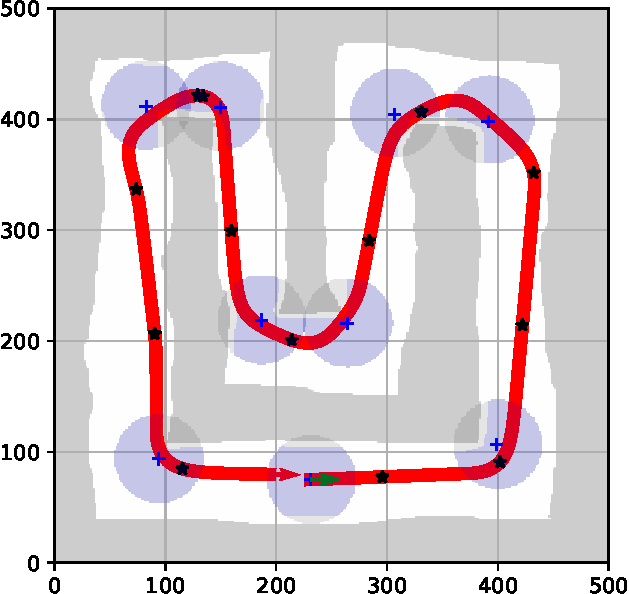
\includegraphics[width=\textwidth]{../img/experiments/u-hybrid_astar-trajectory}
		\end{subfigure}
		\hfill
		\begin{subfigure}[t]{0.45\textwidth}
			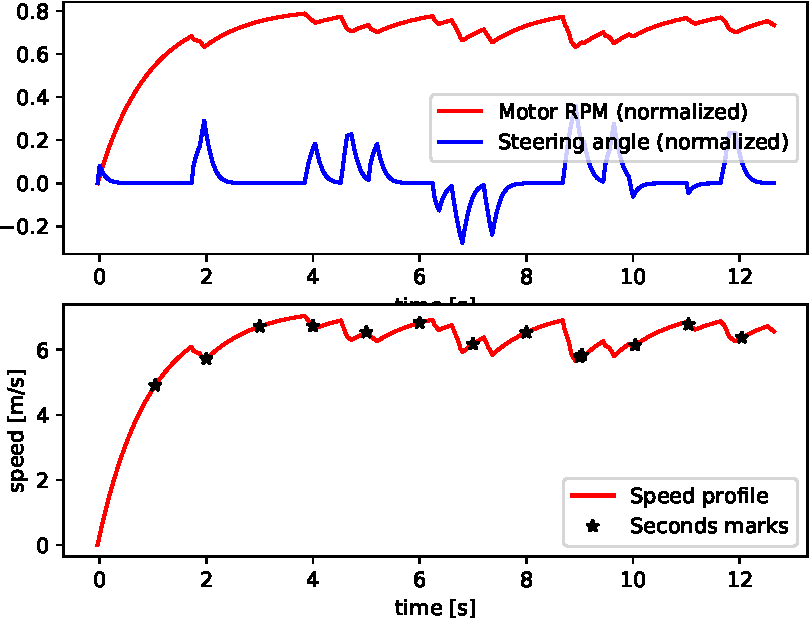
\includegraphics[width=\textwidth]{../img/experiments/u-hybrid_astar-actuators}
		\end{subfigure}	
		\caption{Solution found by Hybrid A* in \SI{440.10}{\milli\second}}
		\label{fig:u-hybrid_astar}
	\end{subfigure}

	\vspace{0.75cm}

	\begin{subfigure}[t]{\textwidth}
		\begin{subfigure}[t]{0.45\textwidth}
			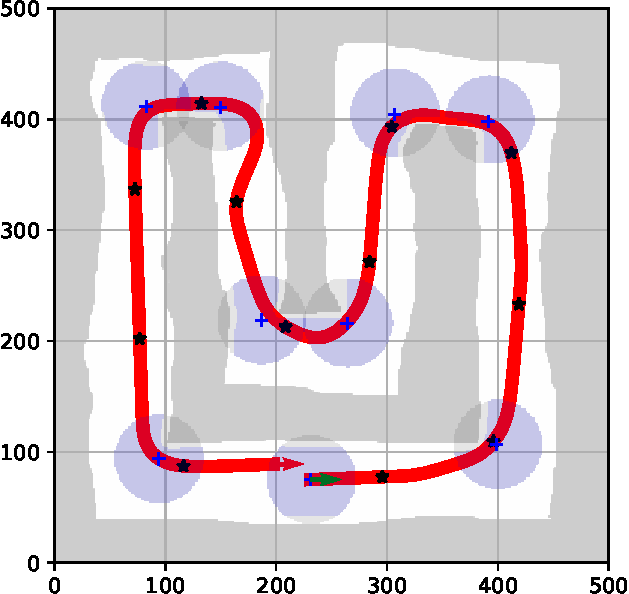
\includegraphics[width=\textwidth]{../img/experiments/u-sehs-trajectory}
		\end{subfigure}
		\hfill
		\begin{subfigure}[t]{0.45\textwidth}
			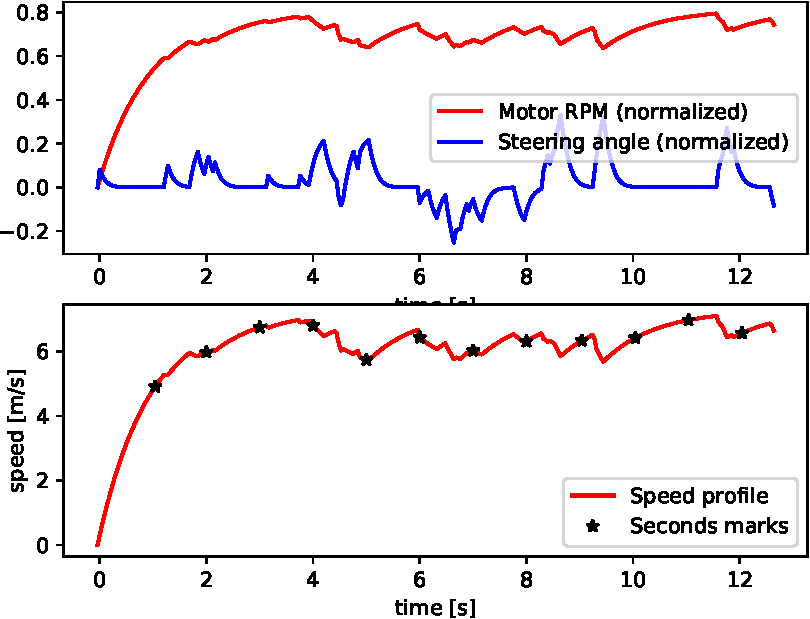
\includegraphics[width=\textwidth]{../img/experiments/u-sehs-actuators}
		\end{subfigure}
		\caption{Solution found by SEHS in \SI{533.60}{\milli\second}}
		\label{fig:u-sehs}
	\end{subfigure}
	
	\vspace{0.75cm}
	
	\begin{subfigure}[t]{\textwidth}
		\centering
		\begin{tabular}{r r r r r r r r}%
        \toprule
            Actions & Grid cell size & RPM levels & Heading angle sectors & Opened & Expanded & Search time & Distance & Lap time \\
        \midrule
            \num{44} & \num{1.80} & \num{20} & \num{18} & \bftab \num{145240} & \bftab \SI{440.10}{\milli\second} & \SI{73.18}{\meter} & \SI{23.08}{\second} \\
            \num{84} & \num{1.44} & \num{40} & \num{36} & \num{1442255} & \SI{3667.90}{\milli\second} & \SI{71.11}{\meter} & \SI{21.84}{\second} \\
		\bottomrule
	\end{tabular}
	\caption{Hybrid A*:}
	\label{table:u-hybrid_astar}
    \end{subfigure}

	\begin{subfigure}[t]{\textwidth}
		\centering
		\begin{tabular}{r r r r r r r r}%
		\toprule
            Actions & Circles & RPM levels & Heading angle sectors & Opened & Expanded & Search time & Distance & Lap time \\
        \midrule
            \num{44} & \num{123} & \num{20} & \num{18} & \num{147605} & \SI{533.60}{\milli\second} & \SI{74.67}{\meter} & \SI{23.64}{\second} \\
            \num{44} & \num{123} & \num{40} & \num{52} & \num{829326} & \SI{2289.80}{\milli\second} & \SI{69.97}{\meter} & \bftab \SI{21.60}{\second} \\
		\bottomrule
	\end{tabular}
	\caption{SEHS:}
	\label{table:u-sehs}
	\end{subfigure}
	
	\vspace{0.75cm}
	
	\caption{Circuit ``U''}
	\label{fig:u}
\end{figure}

\begin{figure}[!tbp]%
	\centering

	\begin{subfigure}[t]{\textwidth}
		\begin{subfigure}[t]{0.45\textwidth}
			\includegraphics[width=\textwidth]{../img/experiments/race_track-hybrid_astar-trajectory}
		\end{subfigure}
		\hfill
		\begin{subfigure}[t]{0.45\textwidth}
			\includegraphics[width=\textwidth]{../img/experiments/race_track-hybrid_astar-actuators}
		\end{subfigure}	
		\caption{Solution found by Hybrid A* in \SI{570.30}{\milli\second}}
		\label{fig:race_track-hybrid_astar}
	\end{subfigure}

	\vspace{0.75cm}

	\begin{subfigure}[t]{\textwidth}
		\begin{subfigure}[t]{0.45\textwidth}
			\includegraphics[width=\textwidth]{../img/experiments/race_track-sehs-trajectory}
		\end{subfigure}
		\hfill
		\begin{subfigure}[t]{0.45\textwidth}
			\includegraphics[width=\textwidth]{../img/experiments/race_track-sehs-actuators}
		\end{subfigure}
		\caption{Solution found by SEHS in \SI{598.10}{\milli\second}}
		\label{fig:race_track-sehs}
	\end{subfigure}
	
	\vspace{0.75cm}
	
	\begin{subfigure}[t]{\textwidth}
		\centering
		\begin{tabular}{r r r r r r r r}%
		\toprule
            Actions & Grid cell size & RPM levels & Heading angle sectors & Opened & Expanded & Search time & Distance & Lap time \\
        \midrule
            \num{44} & \num{1.80} & \num{20} & \num{36} & \num{195755} & \bftab \SI{570.30}{\milli\second} & \SI{85.92}{\meter} & \SI{26.64}{\second} \\
            \num{84} & \num{1.80} & \num{80} & \num{36} & \num{1450767} & \SI{2749.70}{\milli\second} & \SI{82.33}{\meter} & \SI{25.48}{\second} \\
		\bottomrule
	\end{tabular}
	\caption{Hybrid A* peformed worse when compared to SEHS for this track.}
	\label{table:race_track-hybrid_astar}
    \end{subfigure}

	\begin{subfigure}[t]{\textwidth}
		\centering
		\begin{tabular}{r r r r r r r r}%
		\toprule
            Actions & Circles & RPM levels & Heading angle sectors & Opened & Expanded & Search time & Distance & Lap time \\
        \midrule
            \num{44} & \num{164} & \num{20} & \num{18} & \bftab \num{169002} & \SI{598.10}{\milli\second} & \SI{82.66}{\meter} & \SI{25.52}{\second} \\
            \num{124} & \num{164} & \num{20} & \num{52} & \num{1277382} & \SI{4809.20}{\milli\second} & \SI{81.46}{\meter} & \bftab \SI{25.04}{\second} \\
		\bottomrule
	\end{tabular}
	\caption{The solution found by the fastest lap time. Of the two solutions with the lowest computation time, the solution found by SEHS has a significantly better lap time.}
	\label{table:race_track-sehs}
	\end{subfigure}
	
	\vspace{0.75cm}
	
	\caption{Circuit ``Race Track''}
	\label{fig:u}
\end{figure}

\begin{figure}[!tbp]%
	\centering
		
	\begin{subfigure}[t]{\textwidth}
		\begin{subfigure}[t]{0.45\textwidth}
			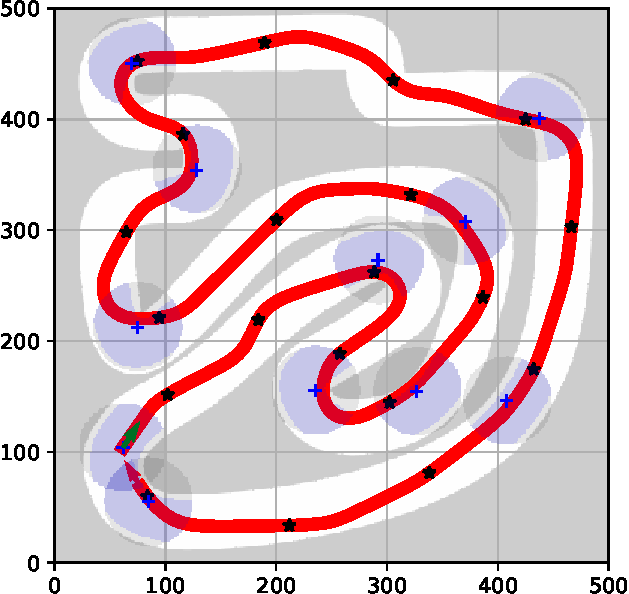
\includegraphics[width=\textwidth]{../img/experiments/zurich-hybrid_astar-trajectory}
		\end{subfigure}
		\hfill
		\begin{subfigure}[t]{0.45\textwidth}
			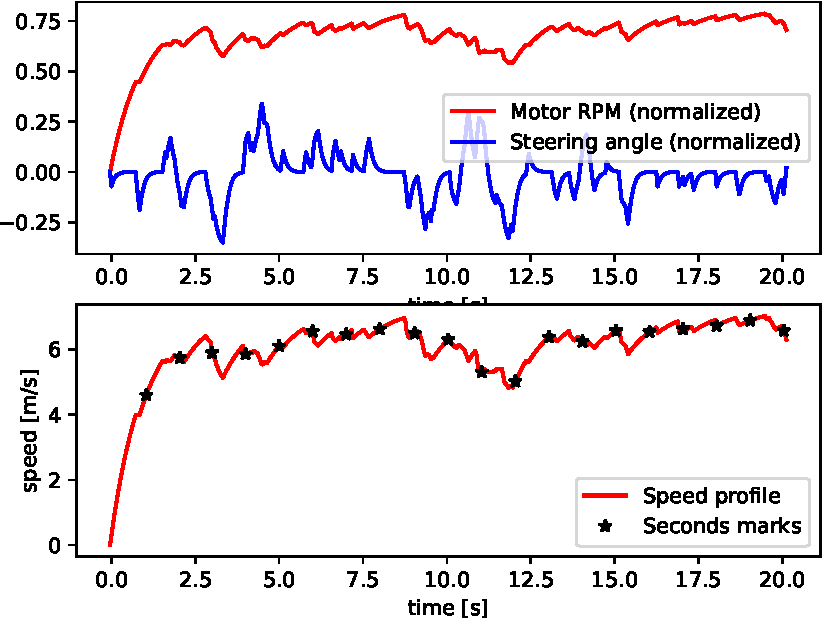
\includegraphics[width=\textwidth]{../img/experiments/zurich-hybrid_astar-actuators}
		\end{subfigure}
		\caption{Solution found by Hybrid A*}
		\label{fig:zurich-hybrid_astar}
	\end{subfigure}

	\vspace{0.75cm}
	
	\begin{subfigure}[t]{\textwidth}
		\centering
		\begin{tabular}{r r r r r r r r}%
            \toprule
                Actions & Grid cell size & RPM levels & Heading angle sectors & Opened & Expanded & Search time & Distance & Lap time \\
			\midrule
                \num{44} & \num{1.80} & \num{40} & \num{36} & \num{488873} & \SI{1041.10}{\milli\second} & \SI{123.67}{\meter} & \SI{41.28}{\second} \\
                \num{88} & \num{1.80} & \num{80} & \num{36} & \num{1922591} & \SI{3811.00}{\milli\second} & \SI{120.09}{\meter} & \SI{38.52}{\second} \\
			\bottomrule
		\end{tabular}
		\caption{Hybrid A* was the only algorithm of the two which found a solution. The SEHS algorithm did not find any solution for any combination of the parameters.}
		\label{table:zurich-hybrid_astar}
    \end{subfigure}
	
	\vspace{0.75cm}

	\caption{Circuit ``Zurich''}
	\label{fig:zurich}
\end{figure}

\section{Limited Lookahead Test}

In this test, we try to compare the performance of the algorithms for a shorter part of the track. For each track, we iterate over the corners we detected using the track segmentation algorithm and we use these corners as initial positions for the search algorithm and let it find a near-time optimal trajectory for the next two and three waypoints.

We want to determine if the algorithms are fast enough to find the following trajectories fast as the car is driving along the circuit. The setup for this test is the same as for the previous test.

\todo[inline]{This part is still not finished.}

\section{Real-World Test}

\todo[inline]{This part is still not finished.}